\begin{figure}[p]
\centering
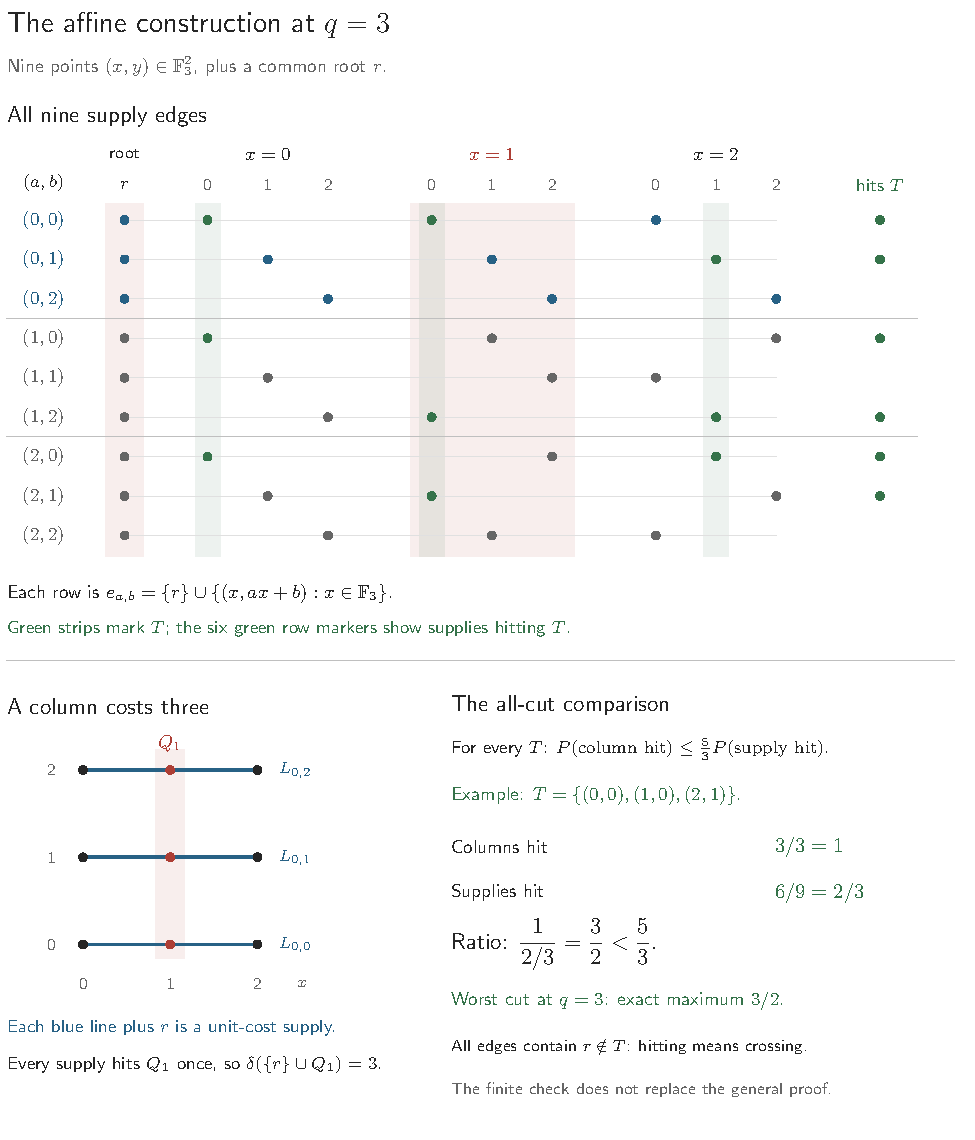
\includegraphics[width=0.97\textwidth]{figures/affine-q3.pdf}
\caption{The construction and hitting comparison at $q=3$.
Every supply contains the root and one point in each column, whereas a
rooted column costs three. The displayed test set hits all three columns
and six of nine supplies, giving ratio $3/2$. Exact enumeration of all
$2^9=512$ test sets (with the empty set handled separately) confirms that
$3/2$ is the maximum for $q=3$, attained by 18 non-collinear triples.
This is a finite check, not a proof for general $q$. The moment bound in
Lemma~\ref{lem:hit} is $C_q=(2q-1)/q$, hence $5/3$ here.
The generator and exact enumeration are included in the repository.}
\label{fig:affine-q3}
\end{figure}
